\documentclass[border=-2pt]{standalone}
\usepackage{tikz}
\usepackage[colorlinks=true]{hyperref}
\usetikzlibrary{decorations.pathreplacing,
  arrows,
  calc,
  decorations.pathmorphing,
  decorations.pathreplacing,
  decorations.markings,
  fadings,
  positioning,
  shapes,
  arrows.meta
}
\tikzfading[name = lens fading,inner color = transparent!0,outer color = transparent!100]
\tikzfading[name = pbs fading,top color = transparent!0,bottom color = transparent!100]
\tikzset{
  mid arrow/.style={postaction={decorate,decoration={
        markings,
        mark=at position #1 with {\arrow[>=stealth]{>}}
      }}},
  mid arrow/.default=0.5,
  mid arrow2/.style={postaction={decorate,decoration={
        markings,
        mark=at position #1 with {\arrow[>=stealth]{><}}
      }}},
  mid arrow2/.default=0.5,
}

\newcommand\drawellipseshade[5][inner color=black,outer color=black]{
  % 1: shading option
  % 2: center (x, y)
  % 3: xsize
  % 4: ysize
  % 5: angle
  \begin{scope}
    \clip[rotate around={#5:#2}] #2 ellipse ({#3} and {#4});
    \begin{scope}[transform canvas={shift={#2}, rotate=#5}]
      \shade[shading=radial,path fading=lens fading, #1] (0, 0) ellipse ({#3} and {#4});
    \end{scope}
  \end{scope}
}
% \newcommand\drawlens[3]{
%   % 1: center (x, y)
%   % 2: size
%   % 3: angle
%   \drawellipseshade[inner color=blue,outer color=blue!40!cyan]{#1}{#2}{{0.14 * #2}}{#3}
% }
% \newcommand\drawwaveplate[3]{
%   % 1: center (x, y)
%   % 2: size
%   % 3: angle
%   \drawellipseshade[inner color=blue!50!black,outer color=blue!80!black]{#1}{#2}{{0.07 * #2}}{#3}
% }
% \newcommand\drawaom[4]{
%   % 1: center (x, y)
%   % 2: xsize
%   % 3: ysize
%   % 4: angle
%   \drawellipseshade[inner color=orange,outer color=orange]{#1}{#2}{#3}{#4}
%   \begin{scope}[rotate around={#4:#1}]
%     \fill[orange, even odd rule, opacity=0.8]
%     ($#1 + ({#2}, 0)$) arc (0:360:{#2} and {#3})
%     -- ($#1 + ({#2}, {#3})$) -- ($#1 + (-{#2}, {#3})$) -- ($#1 + (-{#2}, -{#3})$)
%     -- ($#1 + ({#2}, -{#3})$) --cycle;
%     \draw ($#1 + ({#2}, {#3})$) -- ($#1 + (-{#2}, {#3})$) -- ($#1 + (-{#2}, -{#3})$)
%     -- ($#1 + ({#2}, -{#3})$) --cycle;
%   \end{scope}
% }
% \newcommand\drawpbs[3]{
%   % 1: center (x, y)
%   % 2: size
%   % 3: angle
%   \begin{scope}
%     \begin{scope}
%       \clip[rotate around={#3:#1}] ($#1 - ({#2}, {#2})$) rectangle ($#1 + ({#2}, {#2})$);
%       \begin{scope}[transform canvas={shift={#1}, rotate=#3}]
%         \shade[bottom color=blue!60!cyan, top color=blue!50!cyan, path fading=pbs fading]
%         (-{#2}, -{#2}) rectangle ({#2}, {#2});
%         \draw[line width=1] (-{#2}, -{#2}) -- ({#2}, {#2});
%       \end{scope}
%     \end{scope}
%     % Make sure the frame is not clipped
%     \draw[rotate around={#3:#1}] ($#1 - ({#2}, {#2})$) rectangle ($#1 + ({#2}, {#2})$);
%   \end{scope}
% }
\newcommand\drawlens[3]{
  % 1: center (x, y)
  % 2: size
  % 3: angle
  \begin{scope}[shift={#1}]
    \node[rotate={#3}] at (0, 0) {\scalebox{#2}{
\includegraphics[width=2cm]{imgs/lens.png}}};
  \end{scope}
}
\newcommand\drawwaveplate[3]{
  % 1: center (x, y)
  % 2: size
  % 3: angle
  \begin{scope}[shift={#1}]
    \node[rotate={#3}] at (0, 0) {\scalebox{#2}{
\includegraphics[width=2cm]{imgs/wp.png}}};
  \end{scope}
}
\newcommand\drawaom[4]{
  % 1: center (x, y)
  % 2: xsize
  % 3: ysize
  % 4: angle
  \begin{scope}[shift={#1}]
    \node[rotate={#4}] at (0, 0)
    {\scalebox{#2}[#3]{
\includegraphics[width=2cm,height=2cm]{imgs/AOM.png}}};
  \end{scope}
}
\newcommand\drawpbs[3]{
  % 1: center (x, y)
  % 2: size
  % 3: angle
  \begin{scope}[shift={#1}]
    \node[rotate={#3}] at (0, 0)
    {\scalebox{#2}{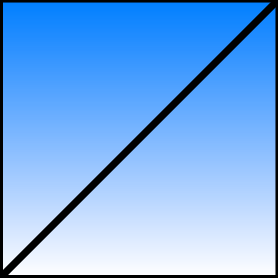
\includegraphics[width=1.4285714285714286cm]{imgs/PBS.png}}};
  \end{scope}
}
\newcommand\drawmirror[4][line width=3]{
  % 1: draw option
  % 2: center (x, y)
  % 3: size
  % 4: angle
  \draw[#1] ($#2 + ({#3 * cos(#4)}, {#3 * sin(#4)})$) --
  ($#2 - ({#3 * cos(#4)}, {#3 * sin(#4)})$);
}

\ifpdf
% Ensure reproducible output
\pdfinfoomitdate=1
\pdfsuppressptexinfo=-1
\pdftrailerid{}
\hypersetup{
  pdfcreator={},
  pdfproducer={}
}
\fi

\begin{document}

\begin{tikzpicture}
  \coordinate (Fiber 1 Out) at (1.1, 0);
  \coordinate (Fiber 1 In) at ($(Fiber 1 Out) + (1.3, 0)$);
  \coordinate (Filter 1) at ($(Fiber 1 In) + (1.5, 0)$);
  \coordinate (Input) at ($(Filter 1) + ({-1.93 * cos(44)}, {1.93 * sin(44)})$);

  \coordinate (DP PBS) at (0, 0);
  \coordinate (Wavemeter) at (0, -2);
  \coordinate (DP AOM) at (-1.7, 0);
  \coordinate (DP lens) at (-4.2, 0);
  \coordinate (DP M1) at (-5.2, 0);
  \coordinate (DP QWP) at (-5.2, 1.4);
  \coordinate (DP M2) at (-5.2 - 0.4, 2.0 + 0.05);
  \coordinate (SP QWP) at (-5.2, 2.4);
  \coordinate (SP IM1) at (-5.2, 4);
  \coordinate (SP lens) at (-6.1, 4);
  \coordinate (SP PBS) at (-7.1, 4);
  \coordinate (SP IM2) at (-9.0, 4);
  \coordinate (SP AOM) at (-9.0, 2.7);
  \coordinate (SP M1) at (-9.0, 0);
  \coordinate (SP M2) at (-7.1, 0);
  \coordinate (SP HWP) at (-7.1, 1.7);

  \coordinate (Servo AOM) at (0, 1.8);
  \coordinate (Fiber 2 In) at (0.3, 3.2);
  \coordinate (Fiber 2 Out) at ($(Fiber 2 In) + (0.5, 0.65) + (-1.7, 0.7)$);
  \coordinate (Pick Off) at ($(Fiber 2 Out) + (-0.5, 0)$);
  \coordinate (Servo PD) at ($(Pick Off) + ({0.8 * cos(30)}, {0.8 * sin(30)})$);
  \coordinate (Filter 2) at ($(Pick Off) + (-1.5, 0)$);
  \coordinate (Output) at ($(Filter 2) + ({2 * cos(44)}, {2 * sin(44)})$);

  \draw[gray!30!white,line width=2] (-4.2, 5.6) |- (-1, 3.3);
  \draw[gray!30!white,line width=2] (1.85, 5.6) -- (1.85, 1.3);

  % Input
  \draw[red,line width=1.6,mid arrow] (Fiber 1 Out) -- (DP PBS);
  % Filter 1
  \draw[red,line width=1.6,mid arrow=0.6] (Filter 1) -- (Fiber 1 In);
  \draw[red,line width=1.6,mid arrow=0.6] (Input) -- (Filter 1);
  \node[red,above] at ($(Input) + (0.6, 0)$) {\large\textbf{From Laser}};

  % Wavemeter
  \draw[red,line width=1.6,mid arrow=0.7] (DP PBS) -- (Wavemeter);
  \node[red,below] at (Wavemeter) {\large\textbf{To Wavemeter}};
  % Between PBS and DP AOM
  \draw[red,line width=1.6,mid arrow2=0.6] (DP AOM) -- (DP PBS);
  \draw[blue,dashed,line width=1.6] (DP AOM) -- (DP PBS);
  \begin{scope}
    % Clip off one arrow
    \clip ($(DP AOM) + (0.85cm, 0.81pt)$) rectangle ($(DP AOM) + (0, 1)$);
    \draw[blue,dashed,line width=1.6,mid arrow2=0.6] (DP AOM) -- (DP PBS);
  \end{scope}
  % Output
  \draw[red,line width=1.6,mid arrow=0.65] (DP PBS) -- (Servo AOM);
  \draw[blue,dashed,line width=1.6] (DP PBS) -- (Servo AOM);
  \draw[red,line width=1.6,mid arrow2] (DP AOM) -- (DP M1);
  \draw[blue,line width=1.6,mid arrow2] (DP AOM) --
  node[above,pos=0.38,rotate=-6] {\small $\approx\!+345~\mathrm{MHz}$} ($(DP M1) + (-0.3, 0.3)$);
  \draw[blue,line width=1.6,mid arrow2] ($(DP M1) + (-0.3, 0.3)$) -- (DP M2);
  \draw[red,line width=1.6,mid arrow2] (DP M1) -- (SP IM1);
  \draw[red,line width=1.6,mid arrow2=0.7] (SP lens) -- (SP IM1);
  \draw[red,line width=1.6] (SP lens) -- (SP PBS);
  \draw[red,line width=1.6,mid arrow=0.6] (SP PBS) -- (SP IM2);
  \draw[red,line width=1.6] (SP IM2) -- (SP AOM);
  \draw[red,line width=1.6,mid arrow] (SP AOM) --
  node[above,rotate=86,pos=0.5] {\small $-80~\mathrm{MHz}$} ($(SP M1) + (-0.2, 0.2)$);
  \draw[red,line width=1.6,mid arrow] ($(SP M1) + (-0.2, 0.2)$) -- (SP M2);
  \draw[red,line width=1.6,mid arrow=0.7] (SP M2) -- (SP PBS);

  % Servo AOM
  \draw[red,line width=1.6,mid arrow=0.65] (Servo AOM) -- (Fiber 2 In);
  \draw[blue,dashed,line width=1.6] (Servo AOM) -- (Fiber 2 In);
  % Pick Off
  \draw[red,line width=1.6] (Fiber 2 Out) -- (Pick Off);
  \draw[blue,dashed,line width=1.6] (Fiber 2 Out) -- (Pick Off);
  \draw[red!50!white,line width=1.2] (Pick Off) -- (Servo PD);
  \draw[blue!50!white,dashed,line width=1.2] (Pick Off) -- (Servo PD);
  \node[right] (Servo Pickoff Node) at (Servo PD) {Servo Pickoff};
  % Filter 2
  \draw[red,line width=1.6,mid arrow] (Pick Off) -- (Filter 2);
  \draw[blue,dashed,line width=1.6] (Pick Off) -- (Filter 2);
  % Output
  \draw[red,line width=1.6,mid arrow=0.6] (Filter 2) -- (Output);
  \draw[blue,dashed,line width=1.6] (Filter 2) -- (Output);
  \node[red,right] at (Output) {\large\textbf{To Tweezer}};
  \begin{scope}
    \clip ($(Output) + (0, 0)$) rectangle ($(Output) + (4, 0.2)$);
    \node[blue,right] at (Output) {\large\textbf{To Tweezer}};
  \end{scope}

  %% Components
  \begin{scope}[shift={($(Fiber 1 Out) + (0.65, 0.5)$)}]
    \draw[line width=1.2]
    (Fiber 1 Out) --
    plot[domain={(-180 - 360 + 90):(180 + 360 + 90)},smooth,variable=\x,samples=2000]
    ({0.5 * cos(\x) + 0.0003 * \x}, {0.5 * sin(\x)}) -- (Fiber 1 In);
    \node[below] at (0, -0.5) {Fiber 1};
  \end{scope}
  \drawmirror[line width=8,gray!60!white]{(Filter 1)}{0.5}{68};
  \node[below] at ($(Filter 1) + (-0.7, -0.45)$) {Filter 1};

  % Input PBS
  \drawpbs{(DP PBS)}{0.7}{0}
  \node[blue!40!cyan,below right] at ($(DP PBS) + (0.2, -0.5)$) {\large PBS 1};
  % DP AOM
  \drawaom{(DP AOM)}{1}{0.4}{90}
  \node[rotate=-90] at (DP AOM) {\large DP AOM};
  % DP Lens
  \drawlens{(DP lens)}{1}{90}
  \node[blue!80!cyan,below] at ($(DP lens) + (0, -1)$-4.5, -1) {\large L1};
  \drawmirror{(DP M1)}{0.9}{-45}
  % DP QWP
  \drawwaveplate{(DP QWP)}{1}{0}
  \node[blue!80!black,right] at ($(DP QWP) + (0.8, 0)$) {\large $\lambda/4$};
  \drawmirror{(DP M2)}{0.3}{3.8}
  % Post DP QWP
  \drawwaveplate{(SP QWP)}{1}{0}
  \node[blue!80!black,right] at ($(SP QWP) + (0.8, 0)$) {\large $\lambda/4$};
  \drawmirror{(SP IM1)}{0.9}{-45}
  % Post DP Lens
  \drawlens{(SP lens)}{1}{90}
  \node[blue!80!cyan,above] at ($(SP lens) + (0, 1)$) {\large L2};
  % SP PBS
  \drawpbs{(SP PBS)}{0.7}{0}
  \node[blue!40!cyan,above] at ($(SP PBS) + (0, 0.5)$) {\large PBS 2};
  \drawmirror{(SP IM2)}{0.9}{45}
  % SP AOM
  \drawaom{(SP AOM)}{1}{0.4}{0}
  \node at (SP AOM) {\large SP AOM};
  \drawmirror{(SP M1)}{0.9}{-45}
  \drawmirror{(SP M2)}{0.9}{45}
  % SP HWP
  \drawwaveplate{(SP HWP)}{1}{0}
  \node[blue!80!black,left] at ($(SP HWP) + (-0.8, 0)$) {\large $\lambda/2$};

  % SP AOM
  \drawaom{(Servo AOM)}{1.2}{0.4}{0}
  \node (Servo AOM Node) at (Servo AOM) {\large Servo AOM};

  \draw[->,>=stealth,green!70!black,line width=0.8,dashed]
  (Servo Pickoff Node) -| (1.7, 2) |- (Servo AOM Node);

  \begin{scope}[shift={($(Fiber 2 In) + (0.5, 0.65)$)}]
    \draw[line width=1.2]
    (-0.5, -0.65) --
    plot[domain={(-180 - 360):(180 + 360 + 90)},smooth,variable=\x,samples=2000]
    ({0.5 * (-cos(\x)-2)}, {0.5 * sin(-\x) + 0.0003 * \x})
    -- (Fiber 2 Out);
    \node[right] at (-0.5, 0) {Fiber 2};
  \end{scope}

  \drawmirror[line width=2,gray!70!white]{(Pick Off)}{0.5}{105};
  \drawmirror[line width=8,gray!60!white]{(Filter 2)}{0.5}{112};
  \node[below] at ($(Filter 2) + (0, -0.45)$) {Filter 2};
\end{tikzpicture}

\end{document}
